An einem Datum werden verschiedene Filme zu bestimmten Uhrzeiten gezeigt.
Jeder Film hat einen Titel und einen Regisseur.\\

\noindent
Erstellen Sie das Domänenmodell inklusive Attributen und Multiplizitäten.\\

\noindent
Welches Muster haben Sie wo und wie verwendet?


\section*{Antwort}
S. Abbildung~\ref{fig:film}.

\begin{figure}
    \centering
    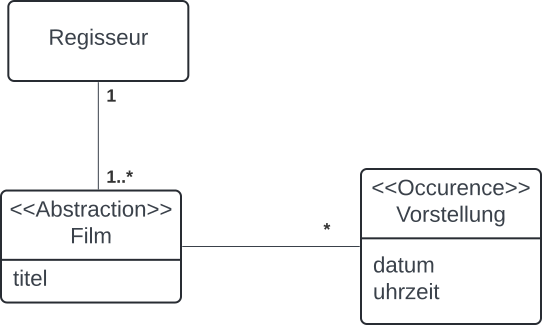
\includegraphics[scale=0.5]{chapters/aufgabe 3/img/film}
    \caption{Domänenmodell für Aufgabe 3. (Quelle: eigene)}
    \label{fig:film}
\end{figure}

\noindent
Anwendung des Musters \textbf{Exemplartyp} für die \code{Film}-\code{Vorstellung}-Assoziation.\\

\noindent
Hierdurch können redundate Informationen in Objekten des Typs \code{Film} vermieden werden: Mehrere Objekte vom Typ \code{Film} hätten sonst identische Attribute wie \code{datum} und \code{uhrzeit}.\\

\subsection*{Anmerkungen}
Im Modellierungsprozess einer ``Vorstellung`` fällt auf: Mehrere Objekte beinhalten für einen Film und seinen \code{titel} gleiche Werte, aber \code{datum} / \code{uhrzeit} unterscheiden sich zwischen den Objekten.\\
Es liegt also nahe, \code{Film} als \textit{Abstraction} zu verstehen, in dem gemeinsame Daten gespeichert werden, und \code{Vorstellung} als \textit{Occurrence}, also das \textit{Auftreten} einer solchen Filmvorführung im gegebenen fachlichen Kontext ``Kino``.\\

\noindent
Ein Objekt vom Typ \code{Regisseur} repräsentiert kein ``Ding``, von dem im Sinne des \textit{Exemplartyp}-Musters gemeinsame Daten in \textit{einem} Objekt, und individuelle Daten (``\code{Film}``) in \textit{weiteren} Objekten festgehalten werden sollen: Objekte vom Typ \code{Regisseur} haben in dem Entwurf eine eindeutige Identität und treten nicht mehrfach auf, wie {bspw.} ein Buch in einer Bibliothek.\\

\noindent
\code{Film} darf also nicht als Auftreten (\textit{Occurrence}) einer \textit{Abstraction} ``\code{Regisseur}`` verstanden werden. Zwar kann ein Film als Werk des Regisseurs auch als Ausdruck seines künstlerischen Schaffens und damit im philosophischen Sinne auch als sein Auftreten verstanden werden: Aber es existieren halt keine ``Kopien`` eines Regisseurs als Person. \\

\noindent
Zur Verdeutlichung wurde noch ein \textit{Assoziationsname} für die Beziehung \code{Regisseur} - \code{Film} (in dieser Leserichtung) angegeben, auch wenn die Semantik aus der Bezeichnung der Klassen hervorgehen sollte.